\chapter{Job control variables}
\label{chp:job-control-variables}
\ProductName{} provides Job control variables for handling all types of dependencies. In this manual, when it is not likely to be ambiguous,
Job control variables are usually just referred to as variables.

There are some variables defined as standard, which are used for controlling the overall operation of \ProductName{}. Other variables may be
created, modified, queried and deleted by any suitably authorised users, via interactive and command line tools.

The specifications for batch jobs include options for interacting with variables before jobs may start, when jobs are starting and when they
finish. For example a job called update may use two variables, called \exampletext{STATUS} and \exampletext{COUNT}, for
dependencies with other jobs and the outside world.

 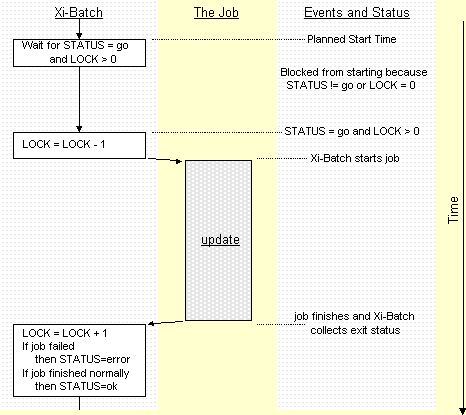
\includegraphics[width=16.925cm,height=14.146cm]{img/ref5.jpg} 

In this example the job \exampletext{update} may not start until the variable \exampletext{STATUS} contains the string
``\exampletext{go}'' and the variable \exampletext{COUNT} contains an integer value less than 10.
In \ProductName{} terminology these tests are called \textit{conditions}. The variables can have their values set by any
combination of the following:

\begin{itemize}
\item \ProductName{} running jobs which specify variable operations for starting.
\item \ProductName{} collecting the exit status of jobs which have finished and specifying variable operations for normal exit, error and/or abort.
\item Users changing the value of variables manually.
\item Batch jobs changing the value of variables themselves.
\item The file monitor program \PrBtfilemon{} setting a variable or variables to indicate the arrival or change of a file.
\item Other processes unconnected with \ProductName{} changing the values of variables via the API or using the command-line tools.
\end{itemize}
Returning to our example, either one or both of the variables do not have the required values, so \ProductName{} waits until both variables meet
the conditions on job update. Once the conditions are met \ProductName{} starts job update running.

When the job finishes, \ProductName{} gets the exit status and performs any specified operations. In this case it will increment
\exampletext{COUNT} by one (however the job finished) and set \filename{STATUS} to ``\exampletext{ok}'' if the job
worked or ``error'' if it did not. In \ProductName{} all operations on variables that are specified in the options
for a batch job are called \textit{assignments}.

Operations on variables are ``atomic''. No other jobs, processes or users can access a variable or variables
whilst they are being tested or changed. This is best seen looking at the assignment of variables \exampletext{STATUS} and
\exampletext{COUNT} when job update finished. Both variables were protected from the time \ProductName{} started incrementing
\exampletext{COUNT} until it finished assigning the appropriate string to \exampletext{STATUS}.

\section{Dependency on files}
Implementation of dependencies based on files is implemented via the \textit{File Monitoring Option}, \PrBtfilemon{},
see page \pageref{btfilemon:startdoc}.

It is not integrated with the main part of \ProductName{} as it is necessary to ``poll'' (repeatedly interrogate at fixed
intervals) the relevant files and directories to monitor for changes.

Typically, \progname{btfilemon} will be set up to modify a variable when the requested file event occurs.

\section{What's in a Variable?}
Apart from having a Name and some Contents, variables also have other pieces of information associated with them. The set of fields which
make up a variable are:

\begin{tabular}{l p{13.5cm}}
Name &
The unique identifier by which the variable is referred to. It is an
alphanumeric string which must start with an alphabetical character.
\ProductName{} will make sure that there are no duplicate or invalid names on
any machine. \\
Value & The information contained by the variable, which can be either an integer value or a text string. \\
Comment & A free text string which should be used to hold a brief description of the variable. \\
User & The name of the user who owns the variable. This is set to the person who created the variable unless it has been transferred to another user. \\
Group & Like the user field this shows which group the variable belongs to. It is set to the primary group of the user who created the variable,
unless it has subsequently been transferred to another. \\
Mode &
Like the modes on a Unix file, these specify who may see and modify the variable. There are, however, far more modes than those associated with
files. Refer to the next section for ``More about Modes''. \\
Export flag &
Variables may be declared as purely local to the machine or accessible by any co-operating \ProductName{} host. This is a binary flag having the
value Local or Exported. Note that two or more hosts may have variables of the same name, the name is distinguished by the host name, thus
host:name. \\
Cluster flag & If a variable is marked ``clustered'' in addition to exported, then a job running on the given host will use
that local version of the variable of that name for conditions and assignments applied to the job.\footnote{\ProductName{} Future versions
of \ProductName{} will make that a feature of a condition rather than a variable.} \\
\end{tabular}
\section{More about Modes}
Access to variables is controlled by the Modes which are similar to Unix file permissions, but with greater functionality. Permission to each
access mode is granted to the owner of the variable (User), users in the same primary group (Group) or everyone (Others).

Here is a screen, from the interactive batch queue management tool \BtqName{}, showing the modes for a variable called A\_STATUS.

\begin{exparasmall}

Modes for Variable {\textasciigrave}A\_STATUS{\textquotesingle}

Variable owner wally group staff

\ \ \ \ \ \ \ \ \ \ \ \ \ \ \ \ \ \ \ \ \ \ \ User \ \ Group Others

Read \ \ \ \ \ \ \ \ \ \ \ \ \ \ \ \ \ \ Yes \ \ \ Yes \ \ No

Write \ \ \ \ \ \ \ \ \ \ \ \ \ \ \ \ \ Yes \ \ \ No \ \ \ No

Reveal \ \ \ \ \ \ \ \ \ \ \ \ \ \ \ \ Yes \ \ \ Yes \ \ Yes

Display mode \ \ \ \ \ \ \ \ \ \ Yes \ \ \ Yes \ \ Yes

Set mode \ \ \ \ \ \ \ \ \ \ \ \ \ \ Yes \ \ \ No \ \ \ No

Assume ownership \ \ \ \ \ \ No \ \ \ \ No \ \ \ No

Assume group ownership No \ \ \ \ No \ \ \ No

Give away owner \ \ \ \ \ \ \ Yes \ \ \ No \ \ \ No

Give away group \ \ \ \ \ \ \ Yes \ \ \ Yes \ \ No

Delete \ \ \ \ \ \ \ \ \ \ \ \ \ \ \ \ Yes \ \ \ No \ \ \ No

\end{exparasmall}

The various modes give the following type of access when permission is granted:

\begin{tabular}{l p{11cm}}
\exampletext{Read} & The variable and its contents can be read.\\
& \\
\exampletext{Write} & The data, name and comment of a variable may be modified.\\
& \\
\exampletext{Reveal} & Variables will be completely invisible to users without reveal
permission. If reveal permission is granted but not read permission
then only the name, owner and group of a variable may be seen. The
contents and comment will be hidden.\\
& \\
\exampletext{Display mode} & Allows these modes to be viewed.\\
& \\
\exampletext{Set mode} & Allows these modes to be changed.\\
& \\
\exampletext{Assume ownership} &
Dictates to whom ownership of a variable may be transferred
relative to the current owner. Hence giving Assume ownership permission
to just the owning User has no value, since the owner can only give the
variable to themselves.\\
& \\
\exampletext{Assume group ownership} &
Dictates to which primary group a variable may be transferred
relative to the current group. Only granting this privilege to Other is
meaningful. User and Group are included to be orthogonal.\\
& \\
\exampletext{Give away owner} &
Grants permission to transfer the ownership of a variable to
another user. The permission may be given to the owner, members of the
same primary group or anyone.\\
& \\
\exampletext{Give away group} &
Grants permission to transfer the variable to another group.
The permission may be given to the owner, members of the same primary
group or anyone.\\
& \\
\exampletext{Delete} & Permission to delete variable from \ProductName{}\\
\end{tabular}

\section{Examples of Dependencies Handled by Variables}
Any job can have several conditions and make several assignments, hence the possibilities for handling dependencies are infinite. This section
contains some examples to help understand the importance of variables.

\subsection{Running Jobs in a Simple Chain}

\begin{figure}
\centering
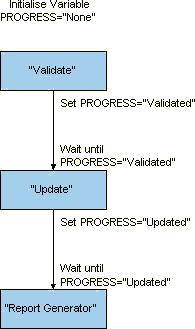
\includegraphics[width=9.019cm,height=14.168cm]{img/ref6.jpg}
\end{figure}
The simplest example of job dependencies is a single threaded chain of jobs, which is controlled by one variable. Each job in the chain is
required to start as soon as possible after the previous job has finished.

To prevent subsequent jobs firing off prematurely the variable, \exampletext{PROGRESS}, must be initialised to some safe value
before the first job starts. Words like ``\exampletext{None}'', ``\exampletext{Ready}'', ``\exampletext{Standby}'' or the
empty string, {\textquotedbl}{\textquotedbl}, are good options.

The most obvious values to use for \exampletext{PROGRESS} are perhaps numeric, since each job could simply increment the value by one.

Using string values has the following advantages:

\begin{itemize}
\item By choosing meaningful names the progress through the chain of jobs can be seen by looking at the value in
\exampletext{PROGRESS}.
\item Only two jobs need their options changing if new jobs are added or
existing jobs are removed from the chain. One job will need a condition
changing and the other an assignment.
\end{itemize}
\subsection{Running jobs in a chain with exception handling}
This is the same simple chain as used in the previous example but with alternative execution paths to run an exception handler if either of
the first two jobs fail. In this case there is one exception handler, but it would be as easy to have a different handler for the Validate
and Update jobs. The value of \exampletext{PROGRESS} is set to a different string depending on the success or failure of the job.

\begin{figure}
\centering
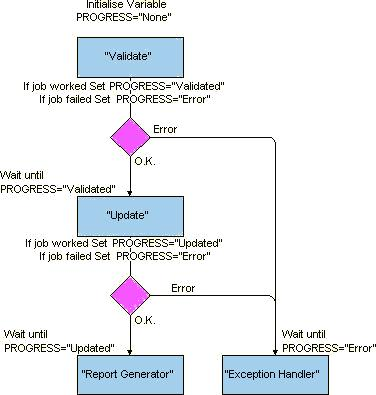
\includegraphics[width=15.854cm,height=14.131cm]{img/ref7.jpg}
\end{figure}
This is a very simple scenario. The exception handler(s) could be programmed to perform recovery actions and resume processing of the
chain at the appropriate job.

Two variables could be used in this example if it is desirable to keep the job exit status separate from the progress through the chain.
\exampletext{PROGRESS} could always be set to indicate the last job that finished. Another variable, for example \exampletext{STATUS},
could be initialised to ``\exampletext{OK}'' and set to ``\exampletext{Error}'' by any job that failed.

\subsection{Running Jobs in Parallel}
A sequence of jobs can contain some that will be running in parallel, to be followed by one or more subsequent jobs. Only one variable is needed
to indicate when all of the parallel jobs have completed.

The variable should be initialised to the number of jobs that will be running concurrently. Each job then decrements this variable by one on
completion. When all of the jobs have finished the value of the variable will be 0.

For example if three jobs are due to run in parallel, using the variable \exampletext{COUNT} then initialise \exampletext{COUNT} to the value of 3.

\begin{figure}
\centering
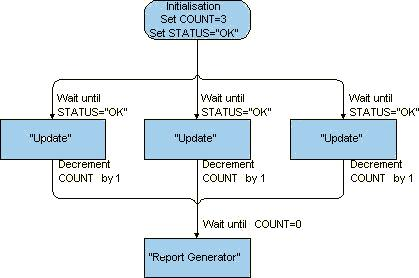
\includegraphics[width=16.743cm,height=11.321cm]{img/ref8.jpg}
\end{figure}

The diagram shows the three jobs waiting for a variable called \exampletext{STATUS} before starting. This is easier to follow
than using \exampletext{COUNT} to control the job start as well.

The value of \exampletext{COUNT} should not be used to indicate the success or failure of the jobs. If this is required then an
additional variable will be needed, as shown in the next section.

\subsection{The Parallel Example with an Exception Handler}
Providing exception handling in a group of parallel jobs will require two variables. One variable will act as a counter to show when all jobs
are completed, as in the previous section. Another variable will be required to show if an error occurred.

The error status variable must be initialised to a value indicating that no errors occurred. Any job which fails should assign an error status
to the variable. All jobs which finish normally must leave the variable alone. For example here is the previous example expanded to use the
variable \exampletext{STATUS} to control whether a Report Generator or an Exception Handler job will run after the three
concurrent Update jobs.

\begin{figure}
\centering
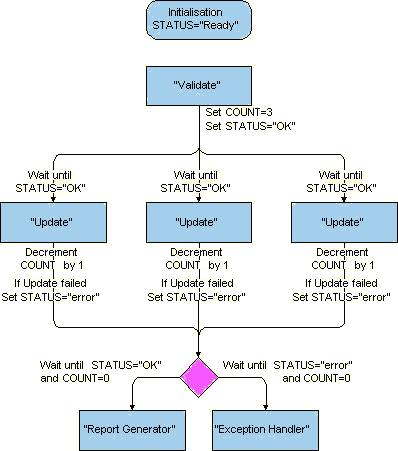
\includegraphics[width=16.378cm,height=16.265cm]{img/ref9.jpg}
\end{figure}
\subsection{Mutual Exclusion \& Semaphores}
It is quite common to find two or more jobs that must never be allowed to run at the same time. This could be because they need the same piece
of hardware, like a particular tape drive. Alternatively they may write to a file or update a database which could be corrupted by being opened
by more than one job.

To enforce the required Mutual Exclusion amongst such a group of jobs, a variable can be used as a semaphore. All jobs in this group are given a
condition that they may only start when the variable has a certain value. They also have an assignment that sets the variable to some
other value on starting and returns it to the initial value on completion.

For example:

Two jobs \exampletext{XYZ} and \exampletext{ABC} can be controlled by one locking variable, called \exampletext{LOCK}.
Both jobs have the condition that \exampletext{LOCK} must be greater than 0. If \exampletext{LOCK} is initialised to 1 then either
job may start when its scheduled start time arrives. The jobs decrement \exampletext{LOCK} on starting and increment
it on finishing, hence \exampletext{LOCK} can only have the values 0 and 1.

\begin{figure}
\centering
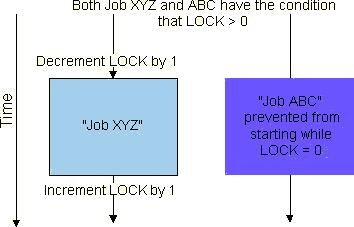
\includegraphics[width=12.838cm,height=8.594cm]{img/ref10.jpg}
\end{figure}
By using the decrement and increment operators in the example we support the general case for limiting the number of concurrently running jobs
to a specific value. In this case 1 enforces mutual exclusion.

If up to a given number of jobs may run at the same time then \exampletext{LOCK} should be initialised to that number. So for a maximum of seven jobs initialise \exampletext{LOCK = 7}.

\subsection{Passing Data between Jobs}
The values of variables can be queried and/or assigned from within a job using the appropriate command line programs (or functions of the API).
This provides enormous flexibility to do the same things between jobs as ordinary variables may do inside them.

For example:


\begin{figure}
\centering
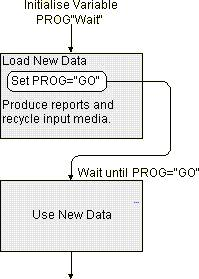
\includegraphics[width=10.746cm,height=11.954cm]{img/ref11.jpg}
\end{figure}
A simple use for setting a Job Control Variable inside a job would be to indicate that the next one in a chain may start before it has finished.

Other operations that can be performed include:

\begin{itemize}
\item Exchanging small amounts of data without using an intermediate file (or possibly the name of a file containing large amounts of data).
\item Providing mutual exclusion between jobs during critical processing rather than for the whole execution of a job.
\item Interrogating variables to see how other jobs have run and are running.
\item Initialising variables to the required values for a particular schedule of jobs.
\item Modifying execution of other jobs in a particular schedule.
\end{itemize}
\section{System variables and logging}
There are seven pre-defined ``System'' variables known to \ProductName{}. They are initially set to be owned by
\batchuser with the default modes which may be reset if desired. These variables may not be deleted or set to an invalid value (e.g. string
for numeric variable etc.). They may be included in job conditions or assignments provided that these do not attempt to perform an invalid
operation on them.

The variables are:

\begin{tabular}{l p{12cm}}
\filename{CLOAD} & \ProductName{} updates \filename{CLOAD} in real time to show the total load level of all currently-running jobs. This is a
read-only variable.\\
& \\
\filename{LOADLEVEL} &
Controls the maximum load of batch jobs that may be running on the system. Jobs can only be started when \filename{CLOAD} is
less than \filename{LOADLEVEL} and it will not put \filename{CLOAD} over the limit set by \filename{LOADLEVEL}.\newline
\filename{LOADLEVEL} may only be set to a numeric value. It may be specified when \ProductName{} is started using the
\exampletext{{}-l} option to \PrBtstart{}, usually to zero, to give maximum control.\newline
If the value is increased, then new jobs may start immediately. If the value is reduced, then it is possible that the total load level of
running jobs may temporarily exceed it until some of them terminate, however no new jobs will start until the level is no longer exceeded.\\
& \\
\filename{LOGJOBS} &
Specifies where to send output from the job audit trail logging. If the variable holds null (an empty data field) then logging is turned off.\\
& \\
\filename{LOGVARS} &
Specifies where to send log output for the variable audit trail. If the variable holds null (an empty data field) then logging is turned off.\\
& \\
\filename{MACHINE} &
This is a read-only variable containing the current machine name, that can only be referenced as a local variable.\\
& \\
\filename{STARTLIM} &
This variable contains the maximum number of jobs that \ProductName{} can start at once. The initial value, upon installation of
\ProductName{}, is 5.\\
& \\
\filename{STARTWAIT} &
This variable contains the waiting time in seconds for the next available job to start if the previous batch set by
\filename{STARTLIM} has not been started for some reason. The initial value upon installation of \ProductName{} is set to be 30 seconds.\\
\end{tabular}
\subsection{Using CLOAD \& LOADLEVEL}
\filename{LOADLEVEL} and \filename{CLOAD} may be used to control the batch workload and avoid conflicts with other activities in a variety of ways.

\warnings{Remember that, in addition to this, each user has a total load level restriction for all the jobs which that user can simultaneously run,
see page \pageref{useradm:loadlevels}.}

\subsubsection{Running fewer batch jobs in office hours}
A batch job can be set up to reduce the value of \filename{LOADLEVEL} at the start of office hours, to prevent
batch jobs slowing down interactive users. Another job can run at the close of office hours to put \filename{LOADLEVEL} back up to
the overnight level.

\subsubsection{Stopping \manualProduct{} gracefully}
To stop \ProductName{}, yet allow jobs to complete, perform the following steps:

\begin{enumerate}
\item Set \exampletext{LOADLEVEL=0}
\item Wait until \exampletext{CLOAD=0}
\item Stop \ProductName{}
\end{enumerate}
This can be done manually or incorporated in a shell script.

It may even be set up as a batch job. However we would recommend that such a batch job has a very low load level, such as 10, much lower than
any other job, and is conditional on \filename{LOADLEVEL} being equal to 10 and \filename{CLOAD} being less than or
equal to 10, so that to start it, all that is required is to set \filename{LOADLEVEL} to 10, and it will automatically wait
until other jobs have finished. At all other times, \filename{LOADLEVEL} would never be set to exactly 10,
\ProductName{} always being restarted with the \exampletext{{}-l} option to \PrBtstart{}.

Batch jobs which stop the scheduler must launch their script asynchronously to avoid killing themselves with the
\PrBtquit{} command. So the actual ``script'' of the job would be:

\begin{expara}

/usr/sbin/batchshutdown \&

\end{expara}

and \filename{/usr/sbin/batchshutdown} would contain

\begin{expara}

\#! /bin/sh

sleep 10

\BtquitName{} -y

\end{expara}

This would give the shutdown job time to complete, before invoking the \BtquitName{} command.

\subsubsection{Starting Administration activities, when Batch work completes}
Set the administration activities up as a batch job to start towards the end of the expected batch work schedule. Specify that
\exampletext{CLOAD=0} as a pre-condition for the administration job. If there are more than one administration jobs to
be run, set them up as a chain of jobs, with only the first one dependant on \filename{CLOAD}.

\subsection{Controlling peak activity}
The variables \filename{STARTLIM} and \filename{STARTWAIT} were created to prevent a large number of
jobs swamping a machine or network by starting at the same instant. For example: if a user scheduled 400 network I/O intensive jobs to start at
Midnight, it is likely that network problems would ensue.

Any process tends to use a large amount of system resources when starting up. If you observe any resource being swamped then lower the
value of \filename{STARTLIM} and/or increase the number of seconds delay specified by \filename{STARTWAIT}.

On high performance machines \filename{STARTLIM} may be increased and/or \filename{STARTWAIT} reduced. The slowest components
may well be any networked or I/O bound resources.

\subsection{Job Logging via LOGJOBS}
This variable may only be set to a string value. It should contain a file name, or a program or shell script name starting with a
``\filename{{\textbar}}''. However, it is vitally important to use ``\filename{{\textbar}}'' with great care so as to ensure the scheduler
process cannot be held up by the receiving process.

If a file name is given, it will be taken relative to the spool directory, by default \spooldir. Thus a file name of \filename{joblog}
will be interpreted, if the spool directory hasn't been changed, as \linebreak[24]\filename{\spooldirname/joblog}.

The file access modes on the file will correspond to the \textit{read/write} permissions on the variable, (execute permissions
will not be set) and the owner and group will correspond to that of the variable, usually \batchuser{}.

If a program or shell script is given, then the \filename{PATH} variable which applied when the scheduler was started (this may be from
the terminal of the user who ran \BtstartName{}) will be used to find the program.

Lines written to the file or sent to the program will take the form

\begin{expara}

03/05/13{\textbar}10:22:43{\textbar}13741{\textbar}date{\textbar}completed{\textbar}jmc{\textbar}users{\textbar}150{\textbar}1000

\end{expara}

Each field is separated from the previous one by a {\textbar}, for ease of processing by \progname{awk} etc. The fields are in the following order (new
versions will add fields on the right):

\begin{center}
\begin{tabular}{l l}
Date & In the form \textit{dd/mm/yy} or \textit{mm/dd/yy} depending
on the time zone.\\
Time & ~ \\
Job Number & Prefixed with host and colon for external jobs\\
Job Title & or if no title {\textless}unnamed job{\textgreater}\\
Status code & (listed below) Prefixed by host and colon if from remote host\\
User & ~ \\
Group & ~ \\
Priority & ~ \\
Load Level & ~ \\
\end{tabular}
\end{center}
The status codes may be one of the following:

\begin{center}
\tablehead{}
\begin{tabular}{|l l|}
\hline
\exampletext{Abort} & Job aborted\\
\exampletext{Cancel} & Job cancelled\\
\exampletext{Chgrp} & Group changed\\
\exampletext{Chmod} & Mode changed\\
\exampletext{Chown} & Owner changed\\
\exampletext{Completed} & Job completed satisfactorily\\
\exampletext{Create} & Job created (i.e. submitted to queue)\\
\exampletext{Delete} & Job deleted\\
\exampletext{Error} & Job completed with error exit\\
\exampletext{force-run} & Job forced to start, without time advance\\
\exampletext{force-start} & Job forced to start\\
\exampletext{Jdetails} & Other details of job changed\\
\exampletext{Started} & Job started\\\hline
\end{tabular}
\end{center}
\subsection{Variable Logging via LOGVARS}
This variable may only be set to a string value. It should contain a file name, or a program or shell script name starting with a
``\exampletext{{\textbar}}''.

If a file name is given, it will be taken relative to the spool directory, by default \spooldir. Thus a file
name of \exampletext{varlog} will be interpreted as the file name \exampletext{\spooldirname/varlog}.

The file access modes on the file will correspond to the \textit{read/write} permissions on the variable, (execute permissions
will not be set) and the owner and group will correspond to that of the variable.

If a program or shell script is given, then the \filename{PATH} variable which applied when the scheduler was started will be used to
find the program, possibly that of the user who ran \PrBtstart{}. Lines written to the file or sent to the program will take the form:

\begin{expara}

03/05/13{\textbar}09:52:43{\textbar}cnt{\textbar}assign{\textbar}Job
start{\textbar}jmc{\textbar}users{\textbar}2011{\textbar}86742{\textbar}myjob

\end{expara}

Each field is separated from the previous one by a ``\exampletext{{\textbar}}'', for ease of processing by \progname{awk} etc.

The fields are in the order(new versions will add fields on the right):

\begin{center}
\begin{tabular}{l l}
Date & in the form \textit{dd/mm/yy} or \textit{mm/dd/yy}, depending on time zone.\\
Time & ~ \\
Variable Name & ~ \\
Status code & (listed below) Prefixed by machine: if from remote host\\
Event code & see below.\\
User & ~ \\
Group & ~ \\
Value & numeric or string\\
Job number & If done from job\\
Job title & if done from job\\
\end{tabular}
\end{center}
The status codes indicate what happened, and may be one of the following:

\begin{center}
\begin{tabular}{|l l|}
\hline
\exampletext{assign} & Value assigned to variable\\
\exampletext{chcomment} & Comment changed\\
\exampletext{chgrp} & Group changed\\
\exampletext{chown} & Owner changed\\
\exampletext{create} & Variable created\\
\exampletext{delete} & Variable deleted\\
\exampletext{rename} & Variable renamed\\\hline
\end{tabular}
\end{center}
The event code shows the circumstance in which the variable was changed, as follows:

\begin{center}
\begin{tabular}{|l l|}
\hline
\exampletext{manual} & Set via user command or operation\\
\exampletext{Job start} & Assigned at job start\\
\exampletext{Job completed} & Assigned at job completion\\
\exampletext{Job error} & Assigned at job error exit\\
\exampletext{Job abort} & Assigned at job abort\\
\exampletext{Job cancel} & Assigned at job cancellation\\\hline
\end{tabular}
\end{center}

